% C13. Curva de decisión del margen en Chapinero (selección adversa)
\begin{frame}{La trampa de Zillow: el vendedor acepta cuando el modelo lo favorece}
  \centering
  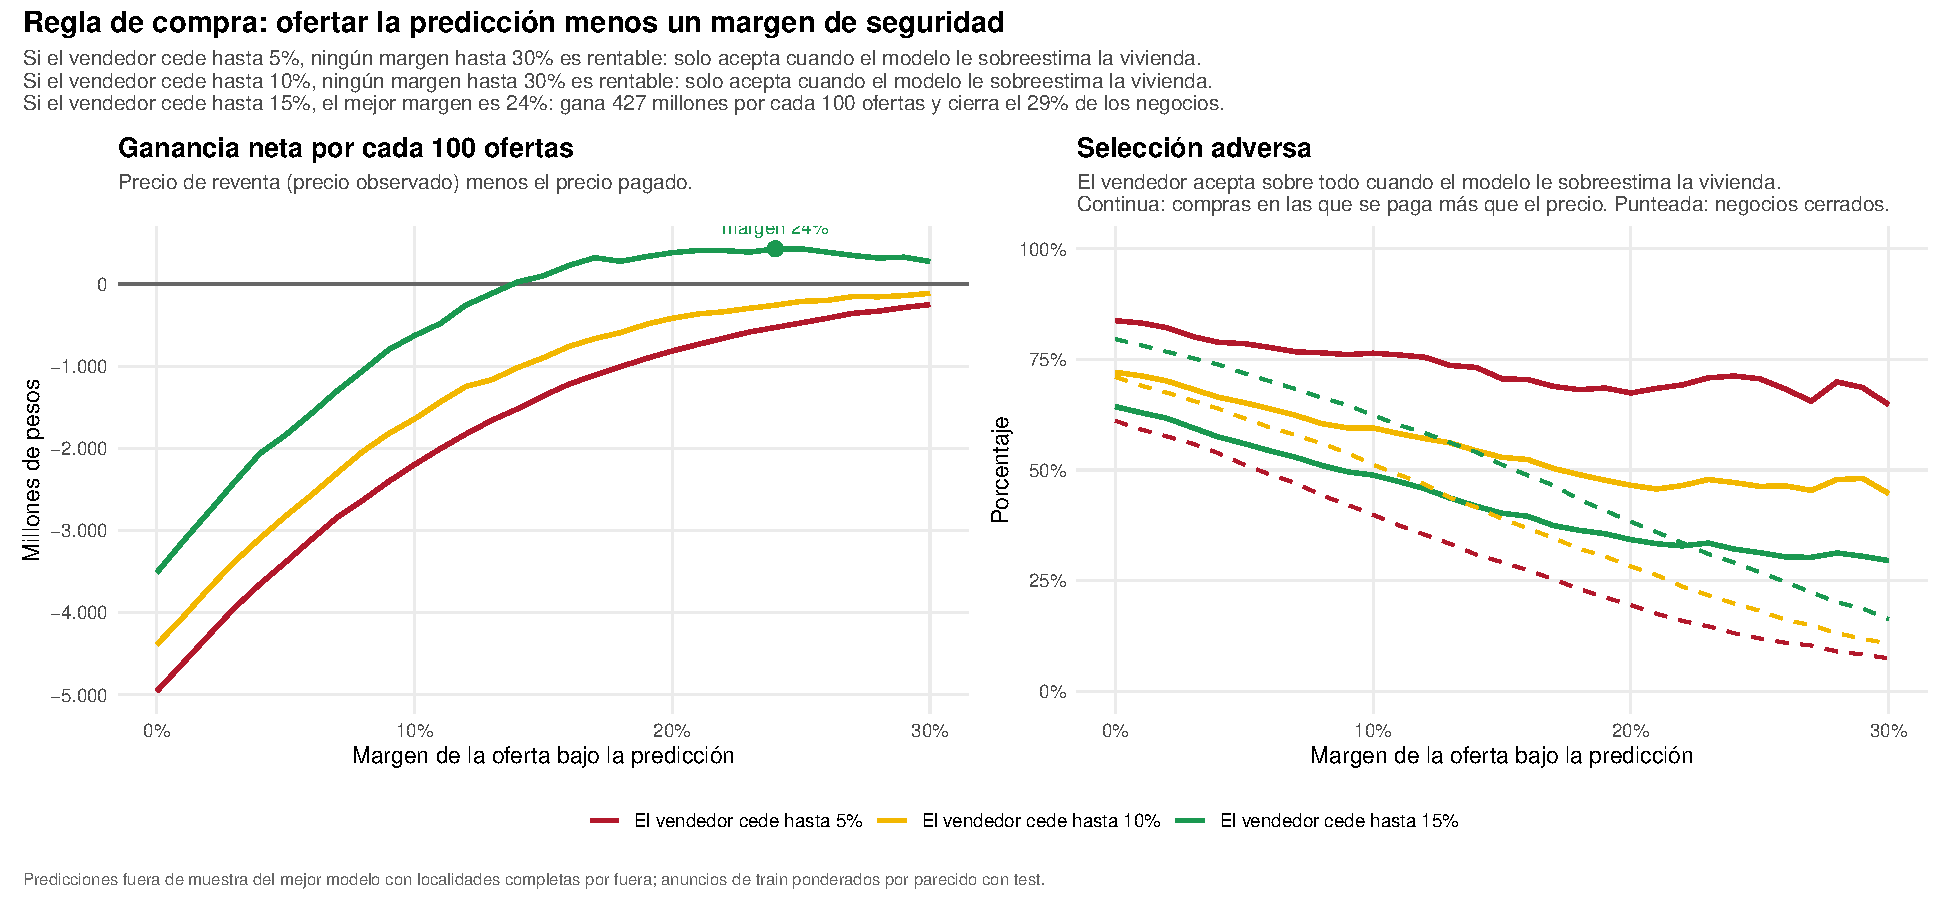
\includegraphics[height=0.8\textheight]{negocio_04_curva_margen.pdf}
  \lectura{En Chapinero, si el vendedor cede hasta \descuentomax, el margen más rentable es \mejormargen{}: \gananciacien{} millones por cada 100 ofertas, cerrando el \negociosmargen{} de los negocios.}
  \note{Selección adversa: los vendedores aceptan nuestra oferta sobre todo cuando el modelo les sobreestima la vivienda, porque en ese caso ofrecemos más de lo que vale. Con descuentos menores, \notadescuentos. Las curvas usan los \nchaptrain{} anuncios de Chapinero en train, por eso no son suaves. Los descuentos que acepta el vendedor son supuestos nuestros, no datos.}
\end{frame}
